\subsubsection{myRocktail}\label{subsubsec:myRocktail}

\paragraph{Aufbau}\label{subsubsec:Aufbau_myRocktail}\mbox{}\\

Bei my Rocktail handelt es sich um eine mietbare Cocktailmaschine, welche die Cocktails mittels eines Roboterarms zusammenmixt. Dabei kann er aus bis zu zwölf Zutaten den gewünschten Cocktail zubereiten. Die Maschine ist mobil aufgebaut und kann mittels Räder verschoben werden. Die Front der Maschine ist halbrund aufgebaut, wobei sich die Getränkeflaschen in dieser Rundung auf der Oberseite befinden. Diese sind mit dem Flaschenhals nach unten montiert, so dass das Getränk mittels automatischer Dosierkappe in das Glas abgefüllt werden kann. In der Mitte des Gerätes befindet sich zudem ein Getränkeauslass, welcher das gewünschte Süssgetränk oder Wasser hinzu mischt. \cite{myrocktail.de_home_nodate}

\newpage
\paragraph{Bedienung}\label{subsubsec:Bedienung_myRocktail}\mbox{}\\

Der Kunde kann mittels eines Touch-Displays das gewünschte Getränk auswählen und stellt dann sein Glas auf den dafür vorgesehenen Platz des Roboterarms. Danach fährt dieser die gewünschten Glaspositionen mit dem Glas an und befüllt dieses mittels den automatischen Dosierkappen mit der gewünschten Menge des Getränks. \cite{myrocktail.de_home_nodate} \cite{cnc_automation_wurfel_myrocktail_2017}


\paragraph{Technische Daten}\label{subsubsec:Technische_Daten_myRocktail}\mbox{}\\

\begin{tabular}{@{}llp{0.6\textwidth}}
    Zeit für einen Cocktail: & : & Eine Zubereitungszeit wird nicht explizit angegeben. Allerdings kann gemäss eines Videos entnommen werden, dass die Zubereitungszeit ungefähr 80 Sekunden dauert. \cite{cnc_automation_wurfel_myrocktail_2017} \\
    \hline
    Anzahl verschiedene Cocktails: & : & Es kann zwischen vier alkoholischen und vier nicht alkoholischen Getränken ausgewählt werden. Dabei besteht jedoch auf Kundenwunsch die Möglichkeit eigene Kreationen zu erschaffen. \\ 
    \hline
    Stromversorgung: & : & Es konnten keine Informationen zur Stromversorgung ausfindig gemacht werden. \\
\end{tabular}

\paragraph{Reinigung}\label{subsubsec:Reinigung_myRocktail}\mbox{}\\

Die Endreinigung wird manuell durch das Servicepersonal durchgeführt. Ob dabei ein automatischer Reinigungsmodus existiert konnte nicht ausfindig gemacht werden. Allerdings wird auf dem Prospekt mit einer einfachen Reinigung geworben. \cite{myrocktail.de_home_nodate}

\begin{figure}[h!]
	\centering
	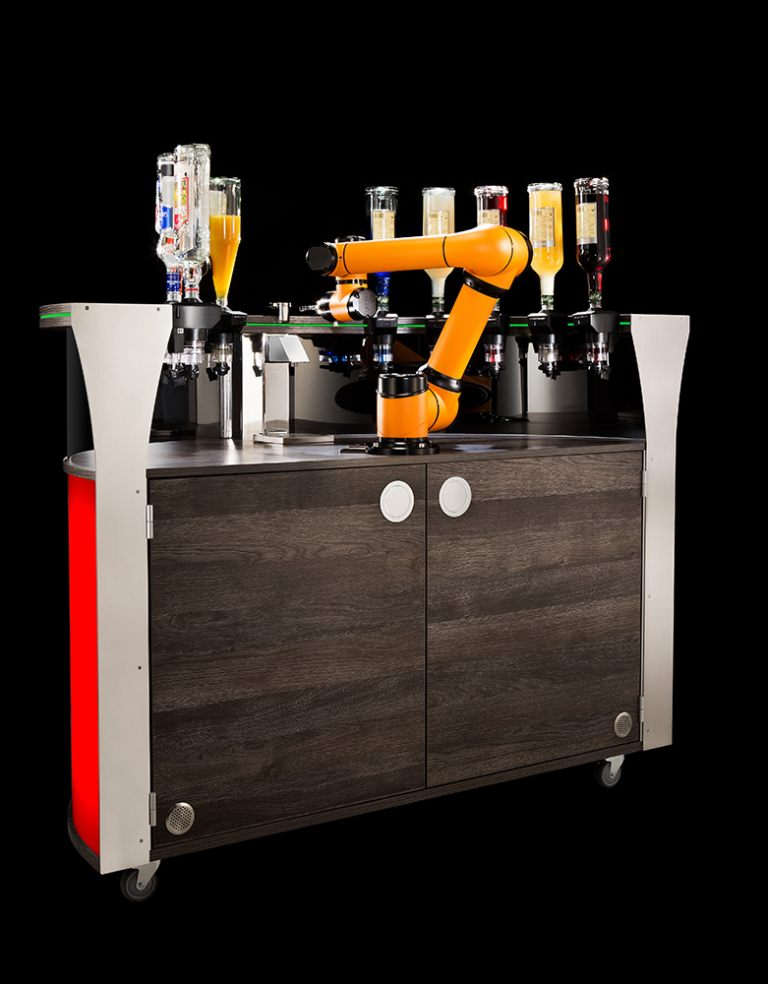
\includegraphics[width=0.3\textwidth]{graphics/myRocktail.jpg}
	\caption{myRocktail \cite{myrocktail.de_home_nodate}}
	\label{fig:myRocktail_Cocktailmaschine }
\end{figure}